\subsection{Giao diện của ứng dụng sau khi đăng nhập}
\subsubsection{Giới thiệu}
Sau khi đăng nhập xong, ứng dụng chuyển sang giao diện chính, đây là nơi người dùng sử dụng các chức năng chính của ứng dụng. Màn hình chính sau khi đăng nhập xong như sau:
\begin{figure}[H]
	\centering{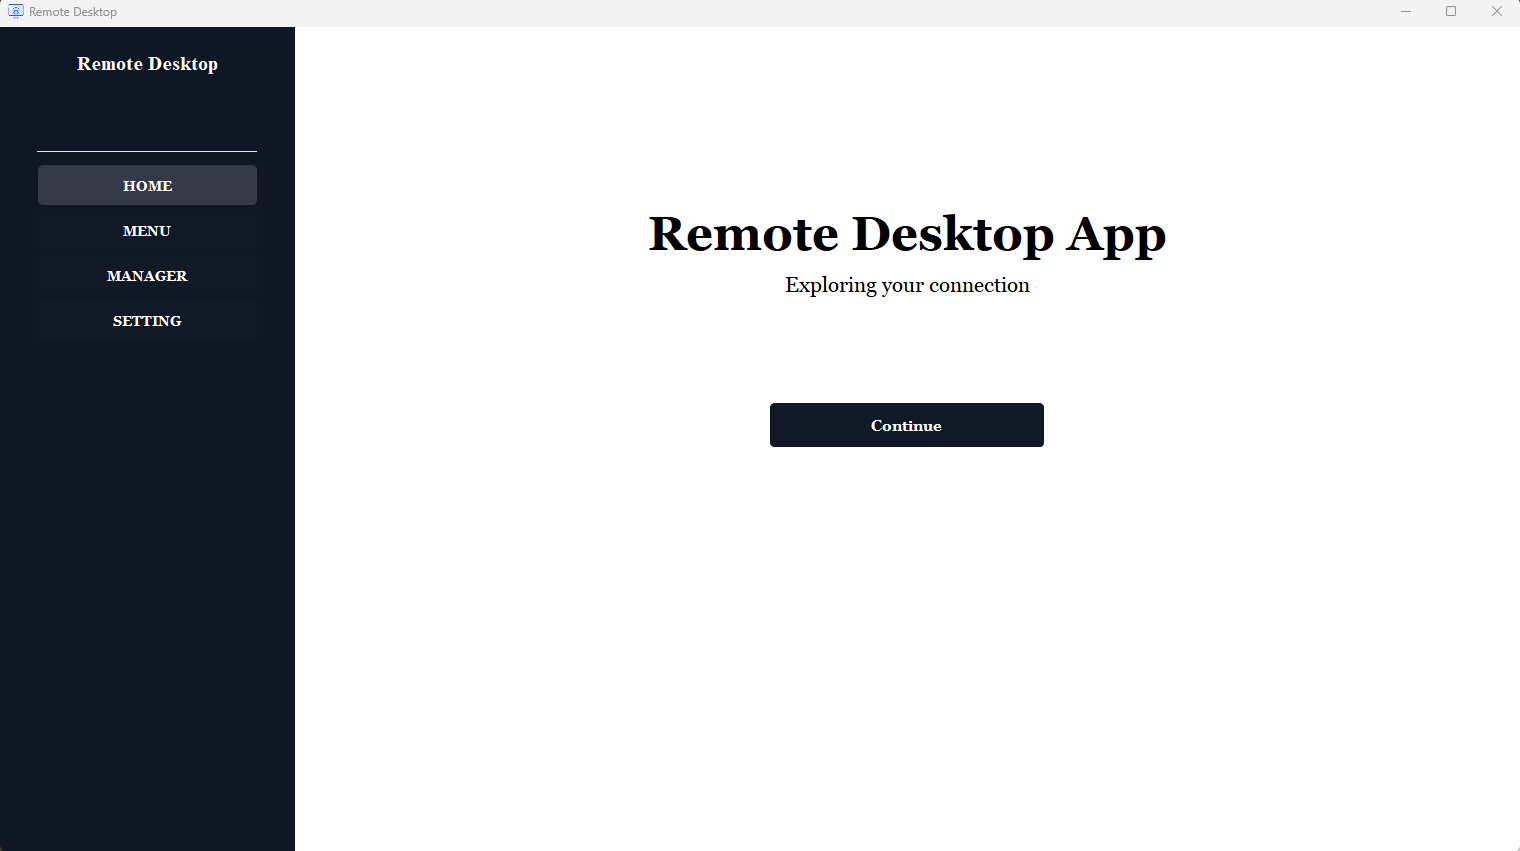
\includegraphics[scale=0.4]{MainWindow}}
	\caption{Màn hình chính của ứng dụng}
	\label{fig:ServerLogin}
\end{figure}
Ở thanh điều hướng, ta có 4 nút chức năng đó là nút \textbf{Home}, \textbf{Menu}, \textbf{Manager}, \textbf{Setting}. Nội dung của màn hình \textbf{Home} là màn hình chính sau khi đăng nhập vừa trình bày ở trên, còn giao diện của các màn hình tương ứng với các nút sẽ được mô tả ở những mục tiếp theo.

Khi người dùng ấn nút Menu trên cửa sổ chính của ứng dụng, ở khu vực hiển thị bên phải sẽ thay đổi tuỳ theo việc người dùng đang đăng nhập với vai trò là \textbf{Admin} (tức \textbf{Client}) hay \textbf{User thông thường} (tức \textbf{Server}).
